\documentclass[tikz,border=12pt]{standalone}
\usepackage[T1]{fontenc}
\usepackage{mathpazo}
\usepackage{amsmath,amssymb}
\usetikzlibrary{arrows.meta, positioning, calc, decorations.pathreplacing}

\definecolor{stblue}{HTML}{7B97AD}
\definecolor{rwgold}{HTML}{B8995E}
\definecolor{sage}{HTML}{7A9A7E}
\definecolor{dkbrown}{HTML}{3D3530}
\definecolor{wmgray}{HTML}{7B7067}
\definecolor{cream}{HTML}{F9F6F0}
\definecolor{border}{HTML}{D4C9B8}
\definecolor{terracotta}{HTML}{C47A6A}
\definecolor{lavender}{HTML}{907EA0}

\begin{document}
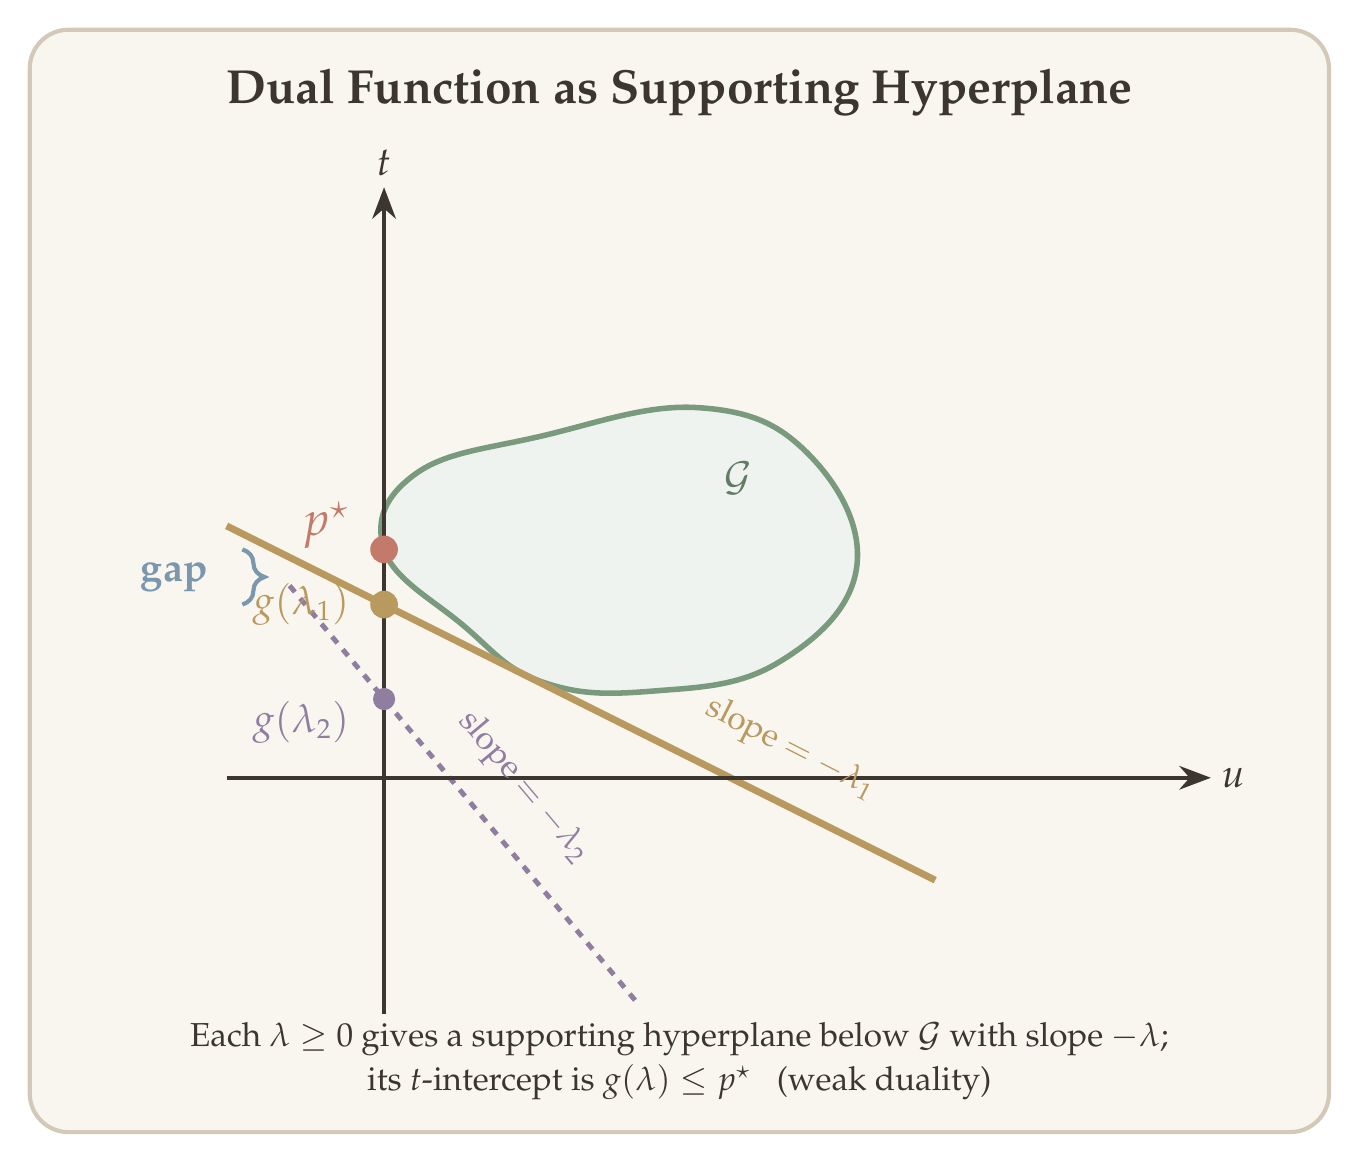
\begin{tikzpicture}[>={Stealth[length=4mm, width=3mm]}, line width=1.5pt]

% Background
\fill[cream, rounded corners=14pt] (-4.5,-4.5) rectangle (12,9.5);
\draw[border, line width=1.5pt, rounded corners=14pt] (-4.5,-4.5) rectangle (12,9.5);

% Title
\node[font=\LARGE\bfseries, text=dkbrown, align=center] at (3.75,8.7)
  {Dual Function as Supporting Hyperplane};

% --- Fills and shapes (drawn BEFORE axes) ---

% The set G
\fill[sage!12, draw=sage, line width=2pt]
  plot[smooth cycle, tension=0.7] coordinates {
    (0,2.9) (1,1.94) (2,1.22) (3.4,1.1)
    (5,1.46) (6,2.66) (5.4,4.1)
    (4,4.7) (2,4.34) (0.4,3.86)
  };
\node[font=\Large\bfseries, text=sage!80!black] at (4.5,3.8) {$\mathcal{G}$};

% Hyperplane 1 (rwgold, tighter bound): slope -0.5, g(lambda_1) = 2.2
% Line: t = 2.2 - 0.5u
\begin{scope}
\clip (-3,-3.5) rectangle (11,8);
\draw[rwgold, line width=2.5pt]
  (-2, {2.2+0.5*2}) -- (7, {2.2-0.5*7});
\end{scope}

% Hyperplane 2 (lavender, looser bound): slope -1.2, g(lambda_2) = 1.0
% Line: t = 1.0 - 1.2u
\begin{scope}
\clip (-3,-3.5) rectangle (11,8);
\draw[lavender, line width=1.8pt, dashed]
  (-1.2, {1.0+1.2*1.2}) -- (3.2, {1.0-1.2*3.2});
\end{scope}

% --- Axes (drawn AFTER fills so they remain visible) ---
\draw[->, dkbrown, line width=1.5pt] (-2,0) -- (10.5,0)
  node[right, font=\Large, text=dkbrown] {$u$};
\draw[->, dkbrown, line width=1.5pt] (0,-3) -- (0,7.5)
  node[above, font=\Large, text=dkbrown] {$t$};

% --- Labels and annotations (drawn last) ---

% Slope labels along visible portions of lines
\node[font=\large, text=rwgold, rotate=-27, anchor=south]
  at (5, {2.2-0.5*5+0.35}) {slope $= -\lambda_1$};
\node[font=\large, text=lavender, rotate=-50, anchor=south]
  at (1.5, {1.0-1.2*1.5+0.45}) {slope $= -\lambda_2$};

% p* point at u=0
\fill[terracotta] (0,2.9) circle (5pt);
\node[font=\LARGE\bfseries, text=terracotta, left] at (-0.3,3.2)
  {$p^\star$};

% g(lambda_1) intercept on t-axis
\fill[rwgold] (0,2.2) circle (5pt);
\node[font=\Large\bfseries, text=rwgold, left] at (-0.3,2.2)
  {$g(\lambda_1)$};

% g(lambda_2) intercept on t-axis
\fill[lavender] (0,1.0) circle (4pt);
\node[font=\Large\bfseries, text=lavender, left] at (-0.3,0.7)
  {$g(\lambda_2)$};

% Brace for gap between g(lambda_1) and p*
\draw[decorate, decoration={brace, amplitude=8pt}, stblue, line width=1.5pt]
  (-1.8,2.9) -- (-1.8,2.2);
\node[font=\Large\bfseries, text=stblue, left] at (-2.1,2.55) {gap};

% Annotation at bottom
\node[font=\large, text=dkbrown, align=center] at (3.75,-3.6)
  {Each $\lambda \ge 0$ gives a supporting hyperplane below $\mathcal{G}$ with slope $-\lambda$;\\[2pt]
   its $t$-intercept is $g(\lambda) \le p^\star$ \; (weak duality)};

\end{tikzpicture}
\end{document}
